\section{Experimental Results}
\label{sec:experimental-results}

	\begin{figure}[b]
		\centering
		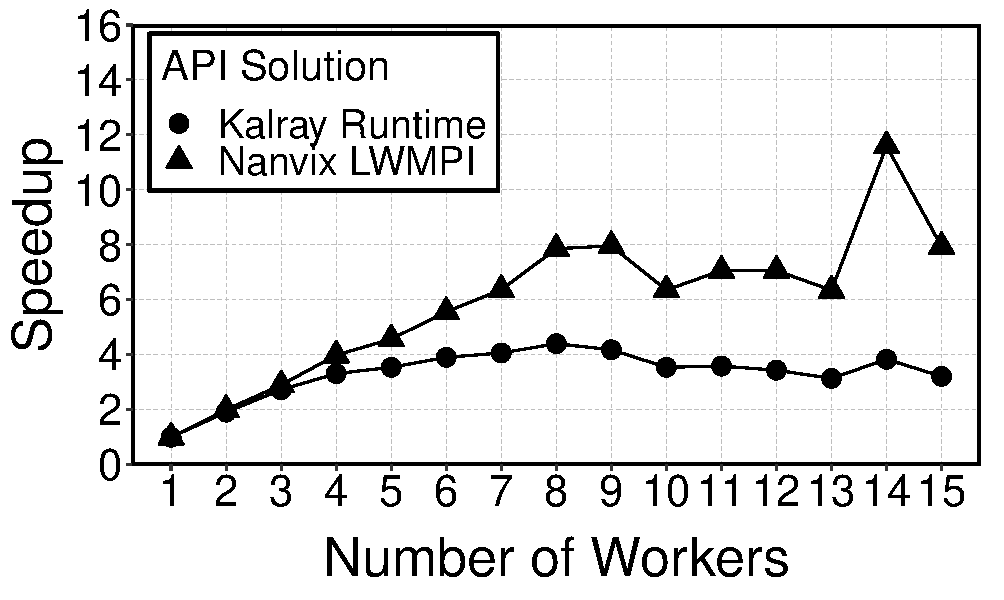
\includegraphics[width=.65\linewidth]{fn-speedup}
		\caption{FN Kernel}
		\label{figure:fn}
	\end{figure}

	% FN
	% Plot Overview
	Figure~\ref{figure:fn} presents the speedup for the FN application.
	%
	% Plot Analysis
	Since FN is CPU-bound, communication has little interference and
	the results show a similar behavior in both solutions.
	%
	% Additional discussion
	The observed behavior is due to the problem design itself and the input workload.
	The leader process performs an integer division to compute the minimum amount
	of work to be sent to each worker. Then, the reminder is added to the last worker,
	which may result in load imbalance. This imbalance is very small up to 8 workers,
	but becomes substantial with more workers. With 14 workers, however, the workload
	is well balanced and the overall performance is improved.
	%
	In general, the results show that \lwmpi scaled well and was able to provide an
	easy adaptation of the kernel without introducing an overhead as the parallelism is
	increased.

	% GF Graphic
	\begin{figure}[t]
		\centering
		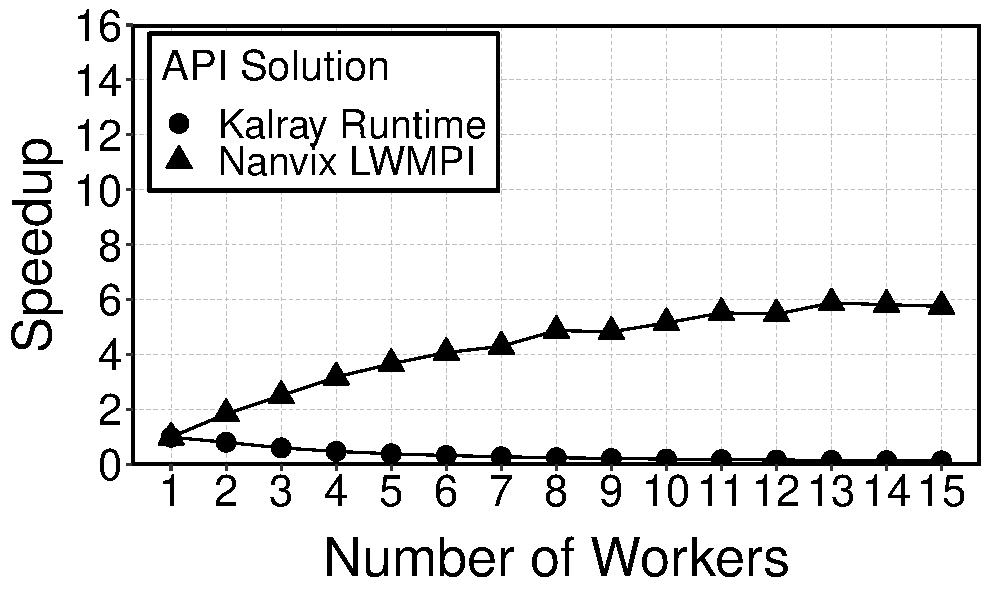
\includegraphics[width=.65\linewidth]{gf-speedup}
		\caption{GF Kernel}
		\label{figure:gf}
		\vspace{-10pt}
	\end{figure}

	% KM Graphic
	\begin{figure}[t]
		\centering
		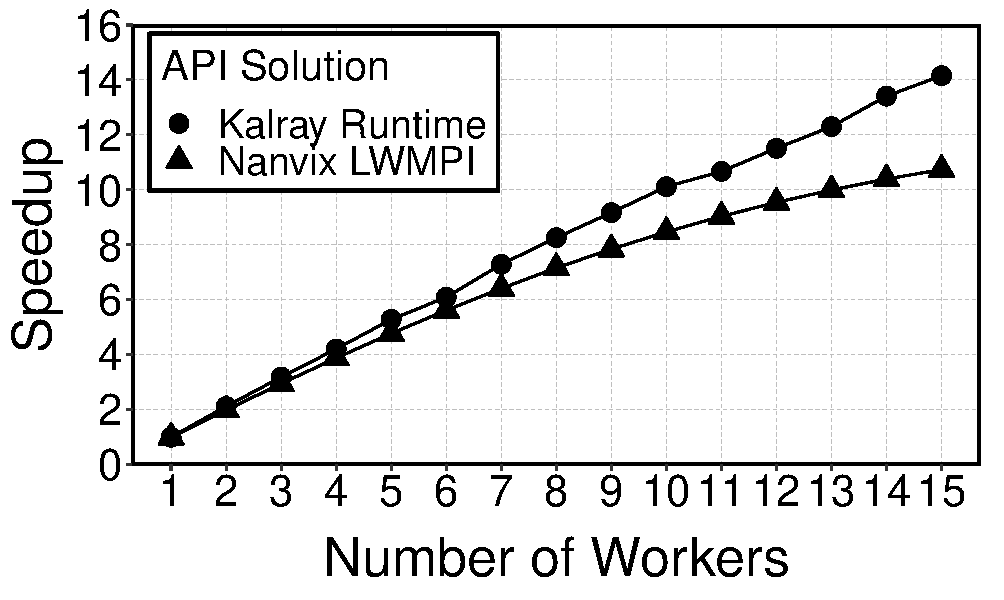
\includegraphics[width=.65\linewidth]{km-speedup}
		\caption{KM Kernel}
		\label{figure:km}
		\vspace{-15pt}
	\end{figure}

	% GF 
	% Plot Overview
	Figure~\ref{figure:gf} pictures the speedup for the GF kernel.
	%
	% Plot Analysis
	As it can be noticed, \lwmpi presented suboptimal scalability whereas
	the default runtime library did not scale at all.
	%
	% Additional discussing
	The small problem sizes may have resulted in insufficient workloads,
	deteriorating the performance of the Kalray runtime.
	At the same time, for \lwmpi this problem seems to be attenuated as
	the parallelism increases, proving its scalability also in these
	situations.
	%
	% Possible improvement
	We believe that using asynchronous communications for both
	solutions would significantly reduce the bottleneck on the leader process
	and improve the overall performance.

	% KM
	% Plot Overview
	Figure~\ref{figure:km} shows the speedup for the KM kernel.
	This application has higher communication demands than the
	previous ones, which impacted the results where \lwmpi achieves lower
	speedups when compared to the Kalray runtime.
	%
	% Additional discussion
	This occurred because the baremetal
	runtime can fitly handle the irregular workload, while \lwmpi is
	limited by the coarse-grained fixed-size messages of the
	\portal abstraction in \nanvix.
	Thus, small problem sizes do not overcome the overhead imposed by
	this abstraction, designed to fit dense data transfers.
	%
	% Possible workaround
	Nevertheless, this situation can be settled by a mechanism that dynamically
	chooses which IPC abstraction fits better the data
	granularity to be sent. It would be possible to use the \mailbox
	abstraction to send fine-grained messages and the \portal abstraction for coarse-grained
	ones. As a result, we could transfer small messages with low latency and large messages
	with high bandwidth.
	%
	% Additional Discussion
	Even so, both solutions had similar linear behaviors, showing that
	\lwmpi was able to keep up with the speedup scalability presented by
	the Kalray runtime.
